\chapter{Related Work}

Designing new systems for collaboration and communication, as opposed to studying existing systems, has long been a major stream of HCI and CSCW research. This section will summarize the most salient past work in this area, although little of this work is recent and responsive to the significant shifts in the way people use technology to communicate, collaborate, and play. 

For a variety of reasons, there has been somewhat of a shift in interest away from the kind of hybrid face-to-face/mediated experiences I create towards building and studying systems for asynchronous experiences between much larger numbers of people. The advent of research on mass collaboration systems like \emph{Wikipedia} (e.g. \citep{Kittur:2007up}) and ``crowd sourcing'' (e.g. \citep{Bernstein:2010wk}) is part of a larger shift away from what was once the center of gravity of systems research. This shift is a natural response to changes in both technology and the common experience of modern collaborative technology users in a web-oriented world where asynchronous interaction became the norm. But the experiences this sort of research studies focus on are predominantly single-channel and asynchronous. This is in stark contrast to my work, which is concerned with the properties of multi-channel synchronous experiences. 

In this work, I focus on interactions within groups both small and large, co-located and remote, but always co-temporal. Although interesting new sorts of work and communication structures are evolving in the asynchronous domain, we should think not just about how to marshal large numbers of people, but about how small groups of people who know each other work, recognizing that much of that work happens face-to-face or co-temporally while geographically distant. It is not effective to treat these interactions as a simple increase in tempo on asynchronous interactions. In synchronous systems, it is much more important to understand how we are perceived (and can control those perceptions) by others. In asynchronous systems, these issues are minimized; we experience others through their actions on shared objects like documents. 

% In my work, I seek to create richer representations of people and better-support person-person interaction instead of person-document-person interaction. 

My survey of related work is organized into three major design strategies: translucence and awareness, adding new communication channels, and design techniques to help people reflect on their own participation and the participation of others. These design strategies have influenced my own design process and have important findings related to my three main research themes: grounding, actions, and attention. As I discuss each design strategy, I will point out their connections to the main research themes. Table \ref{tab:related-work} summarizes the major work covered in this section, and its relationship with the three themes. 


% TODO think about whether to add in a chunk about theoretical perspectives here. Ultimately in the final dissertation there will need to (probably) be a chapter or serious chunk of one laying our theoretical perspecives on grounding, attention, and non-verbal actions. But I don't really want to have to do that now.


% do the table here
% \bullet \medbullet \cdot \filledcircle \filledbigcircle


% c c c c c c c c c c c c c c c c c c c c c

\begin{table*}[tb]
	% \centering

\begin{tabular}{lrcccl}

& & \begin{sideways}Grounding\end{sideways} & \begin{sideways}Actions\end{sideways} & \begin{sideways}Attention\end{sideways} \\
\midrule


\multicolumn{2}{l}{Social Translucence} & & & & \\
\midrule

& \emph{Loops, Babble, Lecture} &$\bullet$& $\CIRCLE$ & $\cdot$ & \citep{Erickson:2000kb} \\
& \emph{Group SketchPad} &$\bullet$& $\CIRCLE$ &$\bullet$& \citep{Gutwin:2002tf} \\
& \emph{CafeCK} &$\bullet$& $\CIRCLE$ &$\bullet$& \citep{Ackerman:1995tj} \\
& Airplane Cockpits & $\CIRCLE$ & $\CIRCLE$ & $\CIRCLE$ & \citep{Hutchins:1995ud} \\
& \emph{ClearBoard} & $\CIRCLE$ &$\bullet$& $\cdot$ & \citep{Ishii:1992bq} \\
\midrule


\multicolumn{2}{l}{Channels} & & & & \\ \midrule & Class Backchannels &
$\cdot$ & $\cdot$ &$\bullet$& \citep{Yardi:2006uk} \\ & Conference
Backchannels & $\cdot$ & $\cdot$ &$\bullet$& \citep{mccarthy_digital_2004} \\
& Semi-Public Displays &$\bullet$&$\bullet$&$\bullet$& \citep{Huang:2003ef} \\
& \emph{Rendezvous} &$\bullet$&$\bullet$& $\cdot$ &
\citep{kellogg_leveraging_2006} \\ & Audio Backchannels & $\cdot$
&$\bullet$&$\bullet$& \citep{Yankelovich:2005bx} \\ & Fragmented Social Mirror
& $\CIRCLE$ & $\bullet$ & $\bullet$ & \citep{Bergstrom:wl} \\ &
\emph{VideoWindow} &$\bullet$& $\cdot$ &$\bullet$& \citep{Fish:1990fn} \\ &
\emph{Thunderwire} & $\cdot$ &$\bullet$& $\CIRCLE$ & \citep{Hindus:1996cn} \\
& \emph{iCom} &$\bullet$&$\bullet$&$\bullet$& \citep{Agamanolis:2003wc} \\ &
\emph{Portholes} &$\bullet$& $\cdot$ &$\bullet$& \citep{Dourish:1992fu} \\ &
\emph{Cruiser} & $\cdot$ & $\CIRCLE$ &$\bullet$& \citep{Fish:1992vz} \\ & GDSS
& $\CIRCLE$ &$\bullet$& $\cdot$ & \citep{nunamaker_electronic_1991} \\ &
\emph{Cognoter} & $\CIRCLE$ & $\CIRCLE$ & $\CIRCLE$ & \citep{Tatar:1991jq} \\
\midrule \multicolumn{2}{l}{Reflection} & & & & \\ \midrule & \emph{Second
Messenger} &$\bullet$& $\cdot$ & $\cdot$ & \citep{DiMicco:2007ie} \\ &
\emph{Meeting Mediator} &$\bullet$& $\cdot$ & $\cdot$ & \citep{Kim:2008ip} \\
& \emph{Conversation Clusters} &$\bullet$& $\cdot$ &$\bullet$&
\citep{Bergstrom:2009fe} \\ & \emph{Conversation Votes}
&$\bullet$&$\bullet$&$\bullet$& \citep{Bergstrom:2009ej} \\ &
\emph{Conversation Clock} &$\bullet$& $\cdot$ &$\bullet$&
\citep{Bergstrom:2007je} \\ \bottomrule \end{tabular} \vspace{3em} \caption{A
summary of the major related work to be discussed in this section and its
relationship with the main research themes. } \label{tab:related-work}
\end{table*}

\subsection{Translucence \& Awareness}

This work owes a clear debt to the work of \citet{Erickson:2000kb} on social translucence. Their work intersects with my action and grounding themes. \emph{Social translucence} is a design strategy that aims to create ``digital systems such that people's presence and activity, made appropriately perceptible, will create accountability and more easily coordinated action''  \citep{Kellogg:2002ts}. They call their example systems designed for this purpose ``social proxies'' that use ``abstract visual representations ... to portray information, in addition to contextual information provided by the other common traces of user activity in mediated communication environments (e.g. persistent conversation).'' In each of their projects (Babble, Loops, Lecture, Auction, etc.; \citep{Erickson:2003td} is a nice overview of these projects), they seek to promote a sense of ``collective awareness'' where each person using the system has a sense of the actions of others in the system and appreciates that this awareness is mutual. 

We share an interest, in my terms, in how we can construct meaningful actions in mediated social spaces and how we can understand how public displays can help ground collaborative and discursive processes. As Erickson and Kellogg point out, this has been a topic of interest both direct and indirect for quite some time in the systems literature. Their work nicely complements work by \citet{Gutwin:2002tf}, who present a framework for thinking about the ways the workspace awareness through actions can be constructed and presented.  \citet{Ackerman:1995tj} shares this interest, too, but focuses on representing overall system activity as an inducement for broader participation. This is an important finding, and one I echo in my work, particularly when it comes to a public, optional system like \emph{backchan.nl}. Distributed cognition, as described by \citet{Hollan:2000ud} represents another productive way to think about these processes; by fostering a sense of mutual awareness we can supporting the kinds of process that \citet{Hutchins:1995ud} describes in flexible communication systems. I see my work as a continuation of these past approaches to representing activity. Although there are many similarities in terms of findings and design strategies, I will focus here on the points of difference as a way to clarify the contributions of my work.

\begin{marginfigure}
	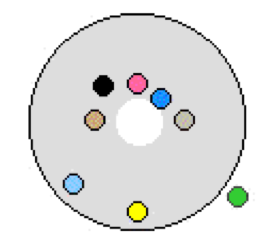
\includegraphics{figures/babble.png}
	\caption{Screenshot of Babble, showing high activity users (in the center) and lower activity users (around the edges), from \citep{Erickson:2003td}.}
	\label{fig:proxy-babble}
\end{marginfigure}

Although Erickson and Kellogg are particularly concerned with what is made visible and what is kept private (the difference between, in their terms, \emph{transparency} and \emph{translucence}), this is a point of divergence between our work. Although I agree with their analysis of the value of considering what actions should be made visible and what should be concealed, it is not a main focus of my analysis. In my work, reading is essentially always invisible and any other action is visible. This is partially a response to their suggestion that it is ``important that participants were aware of the others' awareness of [the properties of the system]'' \citep{Erickson:2003td}. This fits nicely with \citet{Brennan:1991wk}'s presentation of grounding. Simply being told something by someone is not enough for the conversation to move on - you must accept that presentation of information, and that acceptance needs to be accepted by the original presenter. In this way, grounding plays a role not just in communication itself, but in how we communicate information about who we are and what we're doing through actions in the system. 

This finding also suggests that if you don't know which actions are public and which are private, it diminishes the value of translucence as a design strategy. In their work, they tend to rely on physical metaphors to communicate the visibility properties of a system. This is a sensible strategy, but I feel this limits the kinds of experiences we can craft. In my work I tend towards not including invisible actions and instead create completely transparent spaces with carefully selected actions that are worth making visible. This is possible partly because the group sizes in my work are smaller than in the main examples they propose, and it's feasible to show all actions without it being overwhelming. 

\begin{marginfigure}
	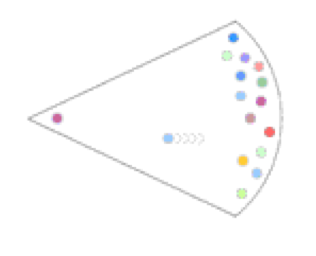
\includegraphics{figures/lecture.png}
	\caption{Screenshot of the lecture proxy, showing the speaker on the left, students on the right, and an interrupting student moving towards the left, from \citep{Erickson:2003td}.}
	\label{fig:proxy-lecture}
\end{marginfigure}

They share a number of specific design findings that complement some of my experiences designing similar systems. They describe three approaches to visualizing activity: realist, mimetic, and abstract. \citep{Erickson:2003td}. I share their interest in abstracted representations, although for different reasons. They argue that realist and mimetic approaches face ``substantial pragmatic barriers (e.g. expense, infrastructure, support)''. In the years since this work was originally done (and well before; one might reasonably argue that \emph{ClearBoard} \citep{Ishii:1992bq} represents an elegant realist approach), many of those pragmatic barriers have fallen. We've seen large-scale virtual worlds (like \emph{Second Life}) that used mimetic approaches and wide adoption of video conferencing which uses realistic representations. Instead, we argue that abstract representations are simply more flexible and better, even given the option of realistic or mimetic approaches.


My work goes into greater depth than Kellogg and Erickson's does on the issue of ``public not personal'' displays. While we agree that it is critical that each person's display doesn't deviate in the kinds of information it represents, in my work these displays are not monolithic---they are not the only venue for interaction between people. Furthermore, displays in my work are most often themselves public, which reinforces the grounding effect. Indeed, that is the most significant deviation between our work. In all of the social proxy work, the proxy is the primary communication medium; in my work, my systems coexist with another primary communication channel, and rarely have any knowledge about the contents of that channel. Public displays also exacerbate issues of attention, which tend not to be major issues for work in the social proxy space (as shown in Table \ref{tab:related-work}). 

% put in a bunch of figures here of the social proxies they designed.



\begin{marginfigure}
	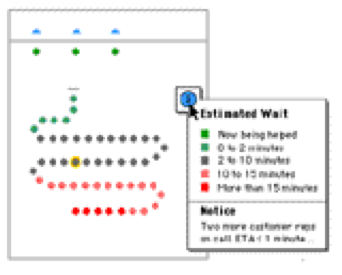
\includegraphics{figures/queue.png}
	\caption{Screenshot of the queue proxy, from \citep{Erickson:2003td}.}
	\label{fig:proxy-queue}
\end{marginfigure}

The other major distinction is in the use of metaphor and display techniques. Erickson and Kellogg box themselves in by limiting their representations to ``a relatively large geometric shape with an inside and an outside and sometimes other features that represent the online situation or context'' \citep{Erickson:2003td} with ``small colored dots'' to represent individual users (similar to \citep{Viegas:1999kv}, minus the direct agency). These design strategies are illustrated in figures \ref{fig:proxy-babble} and \ref{fig:proxy-lecture}. Furthermore, they argue that the best way to represent information is through the use of ``relative movement'' of the user-dots in a way that has ``metaphoric correspondence to the position and movement of people's bodies in face-to-face analogs of the online situation.'' \citep{Erickson:2003td} As I hope my work shows, these limits are not at all necessary to create spaces of meaningful action that facilitate grounded communication and collaboration. Specifically, the need for relying on face-to-face analogs is not a helpful constraint. Instead, my work seeks to create spaces that are easily understood and provide contexts for meaningful action without relying on existing face-to-face metaphors.



\subsection{Channels}

\begin{marginfigure}
	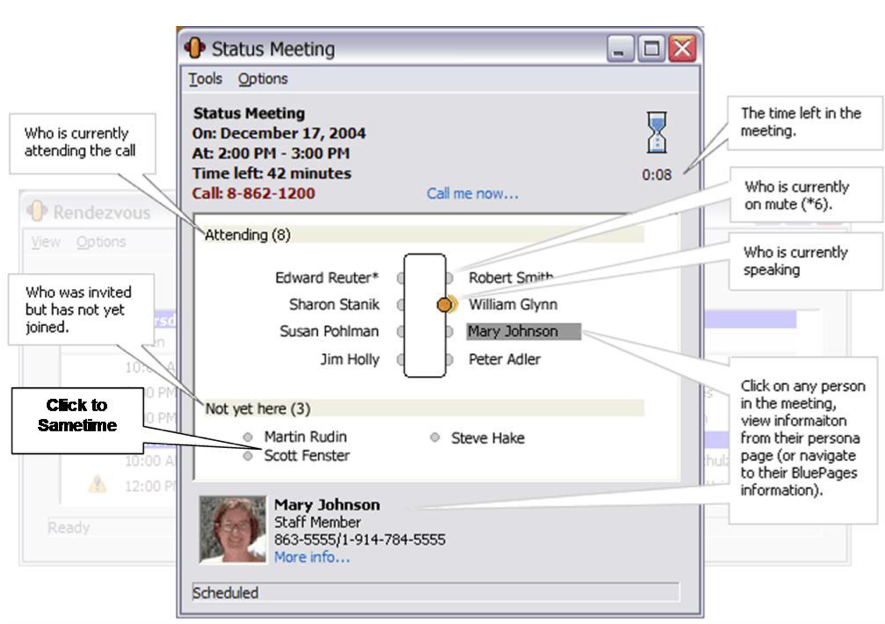
\includegraphics{figures/kellog_social_proxies.png}
	\caption{Screenshot of a meeting-room social proxy for promoting a sense of awareness of other meeting participants, from \citep{kellogg_leveraging_2006}.}
	\label{fig:social-proxies}
\end{marginfigure}

The primary focus of my work is on designing systems that add new communication channels and understanding how those channels operate in contrast to existing channels. In this section, I will present related work that addresses some of these questions.

\begin{marginfigure}
	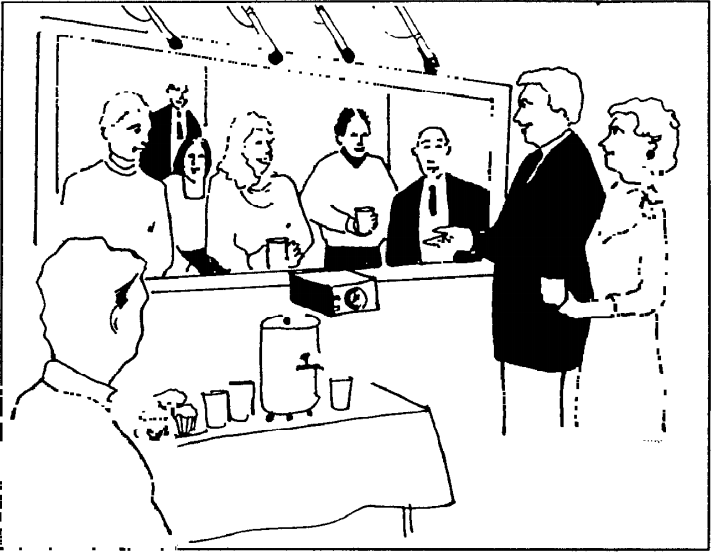
\includegraphics{figures/videowindow.png}
	\caption{Diagram of the VideoWindow scenario for connecting two work-place social spaces, from \citep{Fish:1990fn}}
	\label{fig:videowindow}
\end{marginfigure}

The work most directly related to these questions comes from research into so-called ``backchannels'' in presentation and classroom settings. \citet{Yardi:2006uk} describes how a chat-based backchannel operates over a semester in a classroom, \citet{mccarthy_digital_2004} describe a similar approach at a conference. Backchannels can also be considered a potential part of non-event-oriented contexts too, like long-term co-working among small groups. \citep{Huang:2003ef} Backchannels are not just focused on co-located groups, however, and \citet{kellogg_leveraging_2006} (among others, e.g.  \citep{Yankelovich:2005bx}) has addressed how text and audio backchannels can coexist in distributed contexts. Although past work has addressed in general terms the different ways people use backchannels, it has not sufficiently explained the complicated issues around channel selection, attention, distraction, and identity. Furthermore, in my work I try to move beyond just adding new text or audio channels by adding other kinds of non-verbal actions. In terms of my research themes, past work on backchannels has largely focused on characterizing use patterns, with some discussion of attention. More recent work, like \citep{Bergstrom:wl}, shares an interest in how we can construct actions and how shared displays can be used to help ground the interaction.

\begin{marginfigure}
	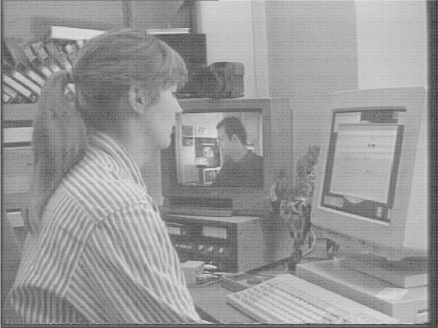
\includegraphics{figures/CRUISER.png}
	\caption{Photo of a CRUISER station installed in an office, from \citep{Fish:1992vz}.}
	\label{fig:cruiser}
\end{marginfigure}

\begin{marginfigure}
	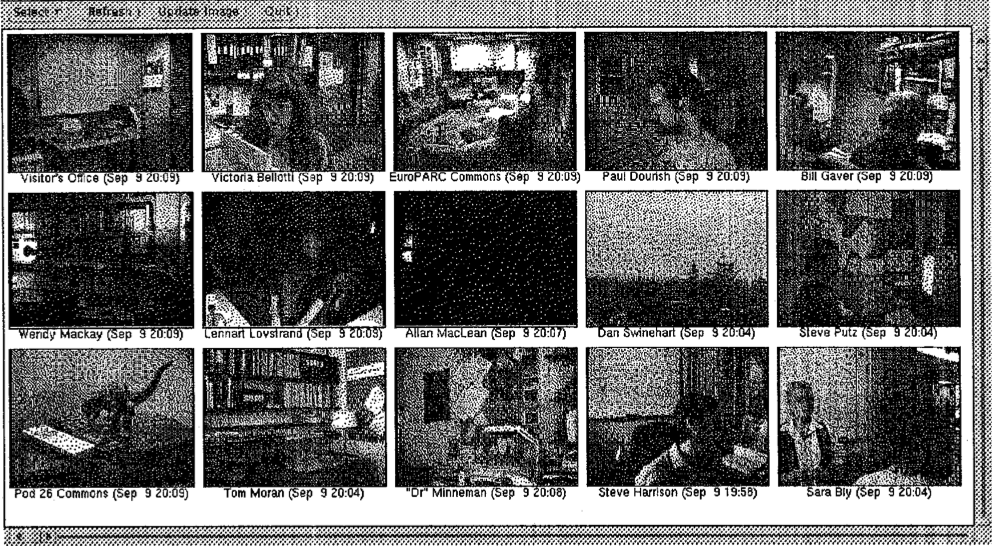
\includegraphics{figures/portholes.png}
	\caption{Screenshot of the Portholes interface, showing periodic stills from a wide range of environmental cameras in an office environment, from \citep{Dourish:1992fu}.}
	\label{fig:portholes}
\end{marginfigure}


Much of the work on creating shared media spaces, driven by experiments at PARC in the late 1980's and early 1990's is salient to my work. Although in some cases this work focused on creating new primary channels, researchers quickly became attuned to problems of privacy and attention because such systems always co-exist with face-to-face communication, in much the same way they do in systems I design. The earliest work at PARC \citep{Olson:1991vz} focused on creating flexible video connections between offices and conference rooms. Subsequent work focused less on a phone-call-like model where connections are created and ended and shifted towards creating spaces with different affordances. Sometimes these involved connecting multiple individuals together, as in CAVECAT \citep{Mantei:1991ww}; other times researchers focused on creating long term persistent video connections in common areas of distributed research groups in the VideoWindow \citep{Fish:1990fn} project. 


Over time, attention shifted more towards a taking advantage of the possibilities to do more than just create ``being there'' experiences. Some researchers experimented with audio-only spaces \citep{Hindus:1996cn}, finding that video was not required to create a sense of connection and space for users, but that the properties of audio did require audio-specific etiquette and coping strategies for the system to be useful. iCom represented a particularly rich design perspective on connecting spaces  \citep{Agamanolis:2003wc}, recognizing that awareness need not be limited to visual awareness, but can extend to information awareness which can be productively embedded in a media space. This embodies the ``beyond being there'' model best of all the work in this research stream: not just trying to create a transparent window between remote spaces, but making something better than a window could be. Furthermore, these projects also focus more on issues of attention, because they are not necessarily always the primary interaction venue for their users. 

% \begin{marginfigure}
% 	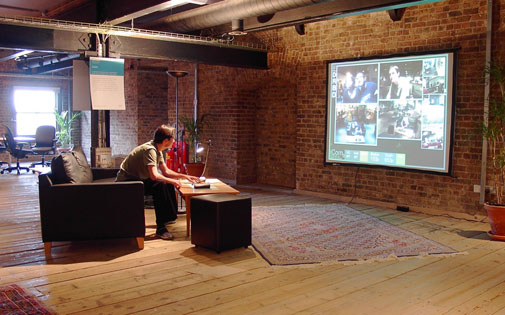
\includegraphics{figures/icom.jpg}
% 	\caption{Photo of one end of an iCom connection, showing multiple video streams and metadata along the bottom of the screen, from \citep{Agamanolis:2003wc}.}
% 	\label{fig:icom}
% \end{marginfigure}


\begin{marginfigure}
	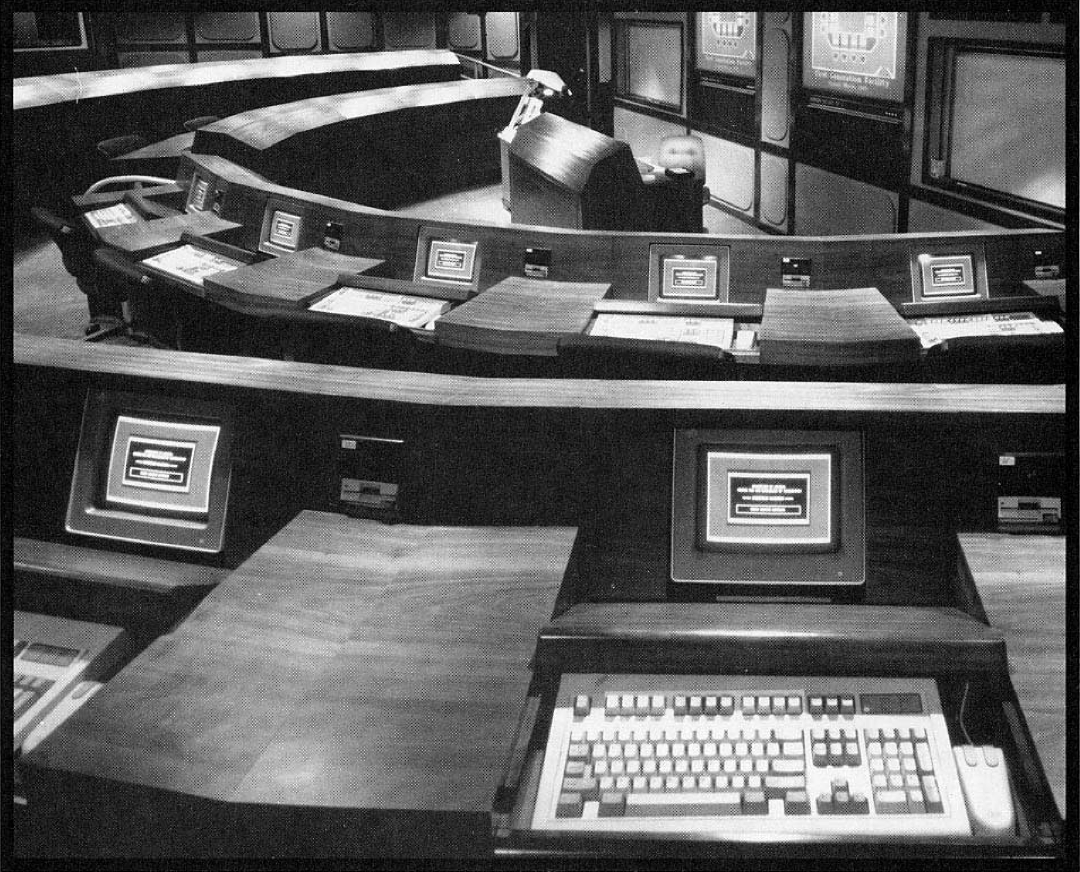
\includegraphics{figures/nunamaker_gdss.png}
	\caption{Photo of a GDSS space, from \citep{nunamaker_electronic_1991}.}
	\label{fig:gdss}
\end{marginfigure}


% also cite karrie's 
% (For subsequent, more artistically inclined approaches to this design space, see Karrie's blah blah, get a nice figure in here for that.)


Serendipity also evolved as an important part of sharing an office environment that was not present with most media space systems. Portholes \citep{Dourish:1992fu} addressed this explicitly by giving people a broader view of remote spaces instead of focusing just on main channel interactions. While my work is not concerned with serendipity, this kind of visual side channel carries important awareness information in much the same way that the side channels in my systems add important contextual information to an interaction. CRUISER \citep{Fish:1992vz} offered non-verbal ways to signal a desire to emulate some of the office hallway etiquette for signaling a desire to drop in and chat informally, without the explicitness of placing a call. The addition of moves like ``cruise'', ``glance'', and ``visit'' are similar in approach to the non-verbal actions at the core of my work like voting in \emph{backchan.nl}, promoting ideas in \emph{Tin Can Classroom}, or moving around the field in \emph{Information Spaces}. 

Early media space researchers proposed a distinction between ``formal'' systems from ``informal'' systems. \citep{Olson:1991vz} While most of the work discussed here (and much of my own work) tends towards the informal side of that continuum, there are some formal elements in my work. This formality manifests most strongly in Group Decision Support Systems research. These systems (exemplified by the work of Nunamaker \citep{nunamaker_electronic_1991}) provide prescriptive systems to support particular brainstorming, decision making, outlining, and voting schemes or policies. In the typical GDSS configuration, each participant has their own computer and interacts with shared structured data in some way, like submitting a new idea or voting on a proposal. In systems like this, the assumption is that having a structured display will ground otherwise informal processes by forcing participants to use the actions the system provides as a set of legitimate conversational moves. Although I tend towards informal systems in my work, the work in this space nonetheless has much to teach us about grounding and actions. 

The lack of consistent results in comparative work in this area \citep{Dennis:1988ww} illustrates the importance of focused design analysis to contextualize findings; it is not useful to view all brainstorming systems as equivalent and comparable in analysis, and I hope that my work will illustrate how the subtleties in interface and approach can have big impacts on outcomes that help explain some of the contradictory results in past GDSS work. Work in this space also raises serious questions related to attention that their work largely fails to address. In fact, in many situations they advocate for largely shutting down pre-existing primary communication channels to focus on the structured, mediated alternative.

Although somewhat rare in the literature, there are a handful of projects that directly address the kinds of hybrid spaces that I seek to create. \emph{Cognoter} \citep{Tatar:1991jq} addresses this design space most clearly. Like my work, \emph{Cognoter} created a hybrid space for very small groups (two to five people) that had both personal and public displays where users could create items and spatially arrange them like on a whiteboard. Textual items can be arranged on a users' display and that arrangement is mirrored on all other users' personal displays. The authors characterize \emph{Cognoter}'s model of creating shared text elements as representing a ``parcel-post'' as opposed to an ``interactive'' conversational model. Instead of embodying a present/accept process (as described by \citep{Clark:1989uc}), they describe their process as being more like literary communication (like email) where the writer tries to make sure ``that the addressees \emph{should have been able} to understand his meaning in the last utterance'' (emphasis mine). This is in contrast to face-to-face interaction, where we can interactively ascertain the extent to which we are being understood (and repair mistakes) before moving on. The authors describe \emph{Cognoter}'s failure to be used effectively by its users as (in part) a conflict between the interactive mode of face-to-face communication and the parcel-post model in \emph{Cognoter}. The \emph{Thoughtswap} project \citep{DickeyKurdziolek:2010wt} also shares my goal in creating hybrid spaces, but like \emph{Cognoter}, the mediated space is used serially with the face-to-face space, while I am interested in creating spaces for legitimate simultaneous performances in mediated and non-mediated spaces. This suggests a major hurdle for my work: can you create systems that use a parcel-post model yet still integrate fluidly with the interactive face-to-face model? \emph{Cognoter} and \emph{Thoughtswap} suggest this is hard, but I will show throughout my work how these barriers can be overcome and suggest ways to explain \emph{Cognoter}'s negative findings.

% go hunting for a desanctis and/or poole piece that's not focusing on AST specifically? also can hit berg if we want, but it feels like a bit of a distraction at the moment.

%, they also produced a nice taxonomy of the kinds of tools that would be useful for distributed collaborative groups: synchronous versus asynchronous communication and open processes versus focused processes, a distinction 


% there's a funny note in the portland paper about how they want to shift away from meeting augmentation to async and task coordination. Funny how times change.

% now summarize. 


% going to want to bring up media equation or whatever that book is called. Cliff Nass. 




% thundewire is just audio, basically a single-channel mumble. not so much about results as describing practices that evolved. 
% portholes is ambient awareness about remote places, not live interaction. cut it?
% videowindow is just like hole in space - audio/video fixed in space

% also mention virtual world stuff? MASSIVE might be worth a quick ref

% "shared media systems"

% - video projects like thunderwire + portholes
% - videowindow


% organize the work in this space 
% projects to talk about:
% - voiceloops
% - backchannel literature
% - social proxies
% - mention conferencing apps
% - Nunamaker
% - zephyr?


% \subsection{Theoretical Perspectives}
% thinking about leaving this out

% stuff from cscw paper:
% systems for reflection
% - second messenger
% - "social mirror" (Karahalios) also bergstrom
% - Meeting Mediator
% 
% systems adding new channels
% - (all the backchan literature: yardi, mccarthy, huang, kellog, yankelovich)
% - do a section on nunameker's work and why it's weird
% - 

% - we'll want to at the very least nod to thinks like voiceloops, and all the audio/video stuff like portholes and thunderwire and that kind of thing. farm my generals reading for that part.
%


% theoretical perspectives
% - practice lens?
% - ethnomethodology? 
% - re-farm wanda's reading list to see what else I can pull from there.

%
% We'll need to do a little organization here. Obviously, farm the references from the Tin Can Edu CSCW paper + backchan.nl paper. We'll need more, ofc, but it's a start. I suspect there will be some ways to separate out systems that allow communication versus those that simply reflect on a main channel. Maybe it's about whether the system itself is a single channel, multi channel, main channel or side channel? 

% write a methodological section here about why it's useful to study this with design work

\subsection{Reflection}

\begin{marginfigure}
	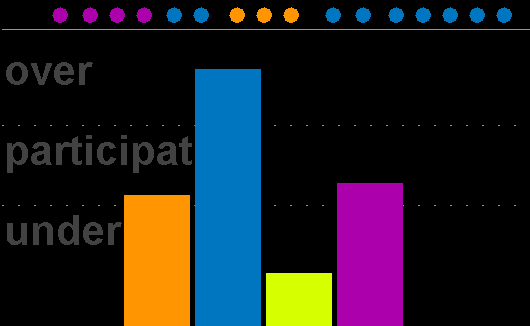
\includegraphics{figures/second-messenger.png}
	\caption{Screenshot of a Second Messenger participation bar-chart, from \citep{DiMicco:2007ie}.}
	\label{fig:second-messenger}
\end{marginfigure}

% \begin{marginfigure}
% 	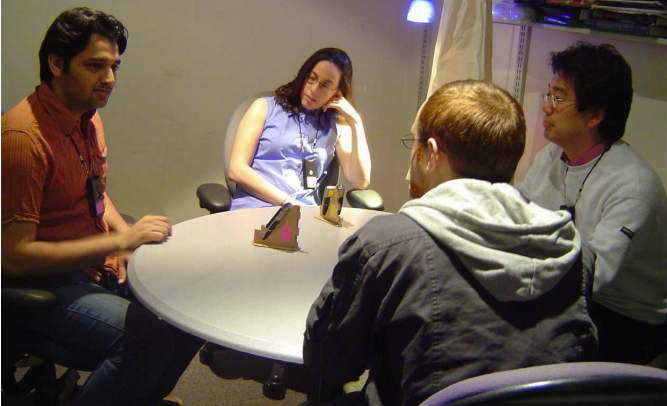
\includegraphics{figures/meeting_mediator.png}
% 	\caption{Meeting mediator.}
% 	\label{fig:meeting-mediator}
% \end{marginfigure}




Understanding how we present ourselves to others has been a topic of sociological inquiry for quite some time. Although many of the insights of scholars like \citet{goffman_presentation_1959} about how we communicate and interpret information about who we are and how we want to be treated are still relevant, the information that is available about people has changed substantially. In some of the examples in this section, designers have added some new bit of information about people to a face to face discussion; in others, we don't have any of the traditional information we would get from being face to face with someone and rely on new types of signals (like the non-verbal actions I propose) to create a sense of people around us. Part of what sets mediated communication apart is the ability to accumulate behavioral histories and represent and reflect those histories to ourselves and others. The work in this space is not as closely connected to my main research themes, but I include it here primarily because it has served as a source of design inspiration. 


\begin{marginfigure}
	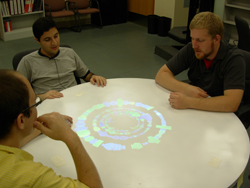
\includegraphics{figures/conversation_clock.png}
	\caption{Photo of Conversation Clock in use, showing relative participation histories from each conversation participant, from \citep{Bergstrom:2007je}.}
	\label{fig:conversation-clock}
\end{marginfigure}

My work is substantially inspired by the work of \citet{DiMicco:2007ie} on the \emph{Second Messenger} project. In this project, participants in a group discussion were presented with a constantly-updating bar-chart visualization representing the relative amount of time they had talked during the discussion. They found that while people who over-participated without a visualization tended to moderate their participation when the visualization was present, people with low participation did not participate more just because others were participating less. \emph{Meeting Mediator} \citep{Kim:2008ip} took a similar approach, but focused on situations where groups of two people could see each other and had to interact with another group of two people who they could only hear. Using a different visualization, Kim et al. found that groups were more interactive with the system than without, although there was not a correlation with group performance. 

\begin{marginfigure}
	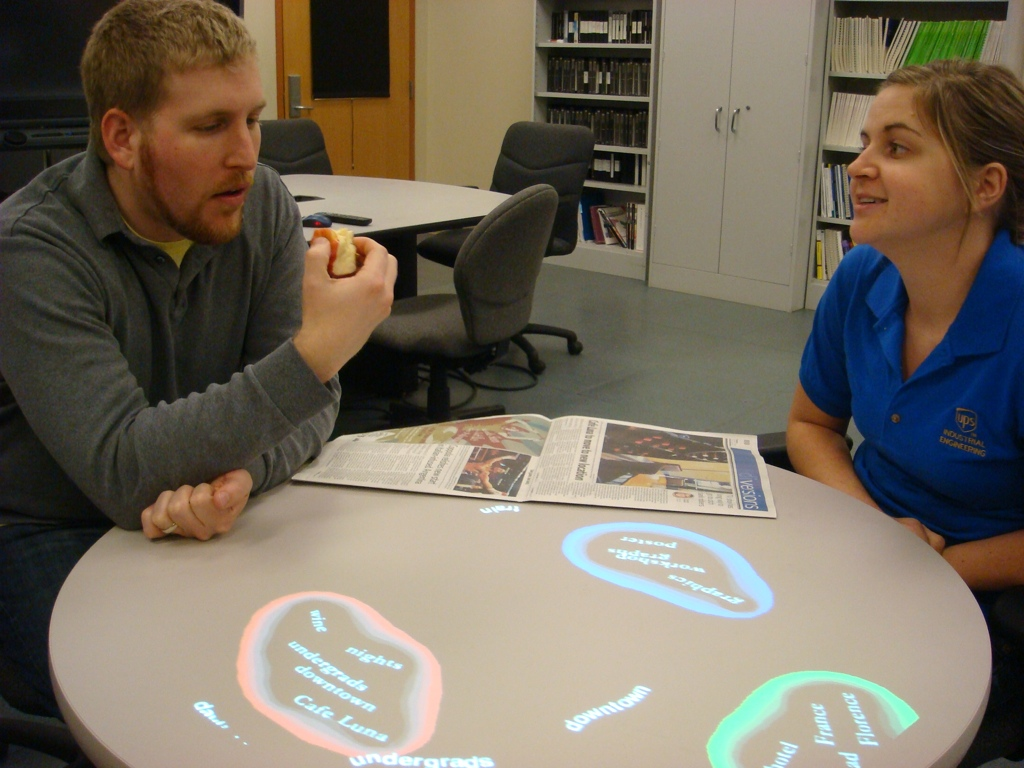
\includegraphics{figures/conversation_clusters.jpg}
	\caption{Photo of \emph{Conversation Clusters}, detecting audio themes and displaying them in visual clusters on the table-top display, from  \citep{Bergstrom:2009fe}.}
	\label{fig:conversation-clusters}
\end{marginfigure}


Bergstrom has done a series of projects that adopt a similar design strategy. \emph{Conversation Clusters} \citep{Bergstrom:2009fe} pulls topics from an audio conversation and presents them in clusters on a table-top display. \emph{Conversation Clock} \citep{Bergstrom:2007je}, like \emph{Second Messenger} and \emph{Meeting Mediator}, visualizes conversation participation, but uses a timeline metaphor instead of a aggregative metaphor. \emph{Conversation Votes} \citep{Bergstrom:2009ej} lets uses discreetly vote about the progress of a discussion, and displays anonymous votes on a table-based display. \citet{Karahalios:hu} describes this design space as ``social mirrors''. 

\begin{marginfigure}
	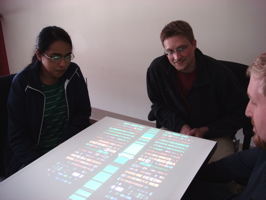
\includegraphics{figures/conversation_votes.jpg}
	\caption{Photo of \emph{Conversation Votes}, showing voting history among conversation participants on the table-top display, from \citep{Bergstrom:2009ej}.}
	\label{fig:conversation-votes}
\end{marginfigure}


% sneak in a \citep{visiphone} here?


% MATT TODO FIX THE MIDDLE OF THIS PARAGRAPH IT'S AWFUL
These are all examples of the accumulate and reflect design strategy, where the system tracks some aspect of behavior: spoken participation in the case of \emph{Second Messenger} and \emph{Meeting Mediator}, discussion topics and group attitudes in the case of Bergstrom's work. 

%The systems then present that information back to the individual or group with the intention that to reflect on and adjust their behavior. Furthermore, all of these projects have an element of grounding to them. By presenting this social information on a shared display (as in my work), it is made salient to the discussion in a way that private displays cannot.

% cite things like last.fm, goodreads, etc in this space?


% \subsection{Identity}

% maybe this whole section is dumb.
% how often do I really deal with this? It's clearly part of the second life work, but not at all part of backchannl, and only a little a part of the Tin Can series. Erm. Move on for now and double back. 

% Many other projects have focused on how peoples' identities are presented. In most of these pieces, there is no face-to-face element, which drives the researcher's interest in developing compelling alternative options that can richly communicate who someone is in a mediated space. Many informal and practical options are in common use; displaying an icon or image chosen by someone and a pseudonym to represent themselves is a widely used design strategy in social applications throughout the internet. These spaces for self expression are frequently augmented by systems that aggregate someone's behavior in that space. This is much like the reflection techniques, but are usually summarizing events beyond any single person's experience. The community site StackOverflow \citep{stack_overflow} provides a particularly rich example of this strategy.

% screenshot a wow forum, stackoverflow, 

% These techniques feel thin compared to the richness of face-to-face interaction, and researchers have developed a number of alternative approaches. Donath's work on data portraiture in a variety of 



% link to things like Ros' work in terms of augmenting face to face interaction with extra information? Or go back to steve mann's cyborg stuff?

% need a paragraph here that's more about the identity side of things. not sure what that will be. chat circles, perhaps? talking in circles? (whichever one had that intersting voting shapes thing)

% how to fit in social proxies and social translucense



% Other potential bits we could fill in here...
% We could spend some time with social translucense
% We could look at non-vebal actions as a space
%	start with Greenbergs stuff, but really look all over for groupware/collaborative tools that had some action to them. Will find some of that in the CVE literature, which might be easy to find
% I don't talk at all about theory stuff here. Could do the spiel about shared displays and grounding, but I'm not sure how critical that is going to be ultimately.
%
%
%  One other strategy is to think about the three research themes: grounding, non-verbal actions, and attention, and go on a hunt for good literature about each of those. 
